\documentclass[
  captions=tableheading,
  bibliography=totoc, 
  titepage=firstiscover,
]{scrartcl}

\usepackage{blindtext} %neuer input

\usepackage{longtable} % Tabellen über mehrere Seiten

\usepackage[utf8]{inputenc} %neuer input

\usepackage{scrhack}

\usepackage[aux]{rerunfilecheck} %Warnung falls nochmal kompiliert werden muss

\usepackage{fontspec} %Fonteinstellungen

\recalctypearea{}

\usepackage[main=ngerman]{babel} %deutsche Spracheinstellung

\usepackage{ragged2e} %neuer input

\usepackage{amsmath, nccmath}

\usepackage{amssymb} %viele mathe Symbole

\usepackage{mathtools} %Erweiterungen für amsmath


\DeclarePairedDelimiter{\abs}{\lvert}{\rvert}
\DeclarePairedDelimiter{\norm}{\lVert}{\rVert}

\DeclarePairedDelimiter{\bra}{\langle}{\rvert}
\DeclarePairedDelimiter{\ket}{\lvert}{\rangle}

\DeclarePairedDelimiterX{\braket}[2]{\langle}{\rangle}{
#1 \delimsize| #2
}

\NewDocumentCommand \dif {m}
{
\mathinner{\symup{d} #1}
}


\usepackage[
  math-style=ISO,
  bold-style=ISO,
  sans-style=italic,
  nabla=upright,
  partial=upright,
  warnings-off={
    mathtools-colon,
    mathtools-overbracket,
  },
]{unicode-math}

\setmathfont{Latin Modern Math}
\setmathfont{XITS Math}[range={scr, bfscr}]
\setmathfont{XITS Math}[range={cal, bfcal}, StylisticSet=1]


\usepackage[
  locale=DE,
  separate-uncertainty=true,
  per-mode=reciprocal,
  output-decimal-marker={,},
]{siunitx}

\usepackage[autostyle]{csquotes} %richtige Anführungszeichen

\usepackage{xfrac}

\usepackage{float}

\floatplacement{figure}{htbp}

\floatplacement{table}{htbp}

\usepackage[ %floats innerhalb einer section halten
  section,   %floats innerhalb er section halten
  below,     %unterhalb der Section aber auf der selben Seite ist ok
]{placeins}

\usepackage[
  labelfont=bf,
  font=small,
  width=0.9\textwidth,
]{caption}

\usepackage{subcaption} %subfigure, subtable, subref

\usepackage{graphicx}

\usepackage{grffile}

\usepackage{booktabs}

\usepackage{microtype} %Verbesserungen am Schriftbild

\usepackage[
backend=biber,
]{biblatex}

\addbibresource{../lit.bib}

\usepackage[ %Hyperlinks im Dokument
  german,
  unicode,
  pdfusetitle,
  pdfcreator={},
  pdfproducer={},
]{hyperref}

\usepackage{bookmark}

\usepackage[shortcuts]{extdash}

%\usepackage{warpcol}

\usepackage{physics}
\allowdisplaybreaks

\begin{document}
    \title{Physik IV Übungsblatt 7}
    \author{  
    Tobias Rücker\\
    \texorpdfstring{\href{mailto:tobias.ruecker@tu-dortmund.de}{tobias.ruecker@tu-dortmund.de}
    \and}{,} 
    Paul Störbrock\\
    \texorpdfstring{\href{mailto:paul.stoerbrock@tu-dortmund.de}{paul.stoerbrock@tu-dortmund.de}}{}
    }
\maketitle
\center{\Large Abgabegruppe: \textbf{4H}}
\thispagestyle{empty}

\newpage
\tableofcontents
\thispagestyle{empty}
\newpage

\setcounter{page}{1}

\section{Aufgabe 1}

    \begin{figure}[H]
        \centering
        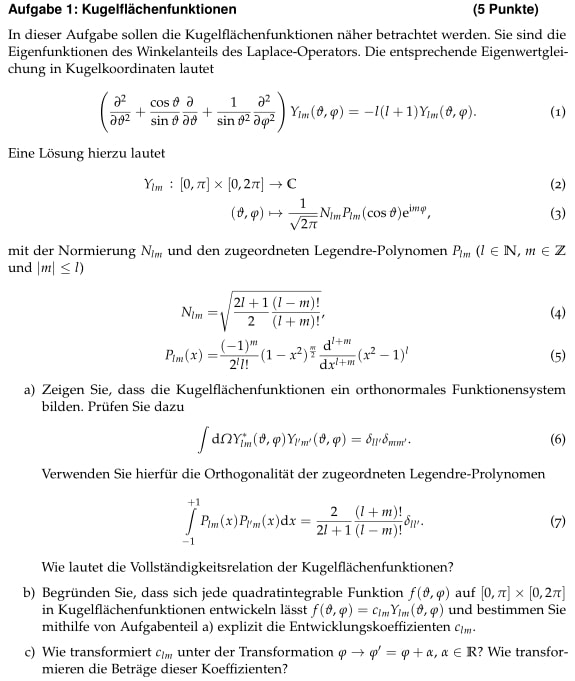
\includegraphics[width=\textwidth]{images/Aufgabe1.jpg}
        \label{fig:1}
    \end{figure}

    \subsection{a)}

    \subsection{b)}

    \subsection{c)}


\section{Aufgabe 2}

    \begin{figure}[H]
        \centering
        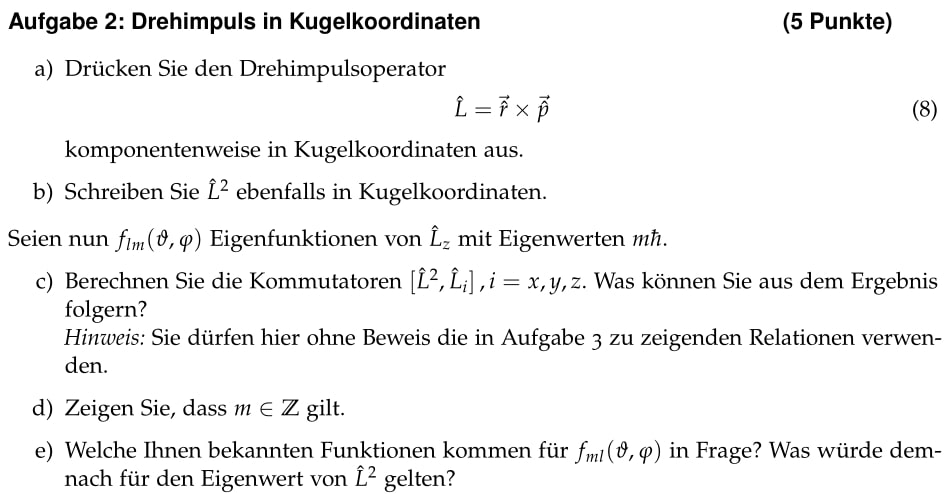
\includegraphics[width=\textwidth]{images/Aufgabe2.jpg}
        \label{fig:2}
    \end{figure}

    \subsection{a)}

    \begin{align*}
    \vec{\hat{L}} &= \vec{\hat{r}} \times \vec{\hat{p}}\\
    L_x &= (yp_z-zp_y)\\
    L_y &= (zp_x-xp_z)\\
    L_z &= (xp_y-yp_x)\\
    \tilde{\vec{r}} &= 
    \begin{pmatrix}
        r\cos(\varphi)\sin(\theta)\\
        r\sin(\varphi)\sin(\theta)\\
        r\cos(\theta)
    \end{pmatrix}\\
    p_x &= -\text{i} \hbar \frac{\partial}{\partial x}\\
    p_y &= -\text{i} \hbar \frac{\partial}{\partial y}\\
    p_z &= -\text{i} \hbar \frac{\partial}{\partial z}
    \intertext{
        \flushleft{Einsetzen\;}\justifying in $L_{x,y,z}$:
    }
    L_x &= -\text{i} \hbar(y\frac{\partial}{\partial z}-z\frac{\partial}{\partial y})\\
    L_y &= -\text{i} \hbar(z\frac{\partial}{\partial x}-x\frac{\partial}{\partial z})\\
    L_z &= -\text{i} \hbar(x\frac{\partial}{\partial y}-y\frac{\partial}{\partial x})\\
    \\
    \frac{\partial \tilde{\vec{r}}}{\partial \varphi} &= \frac{\partial \vec{r}}{\partial x} (-r\sin(\varphi))\sin(\theta) + \frac{\partial \vec{r}}{\partial y} r\cos(\varphi)\sin(\theta)\\
    &= -y \frac{\partial \vec{r}}{\partial x} + x \frac{\partial \vec{r}}{\partial y}\\
    \Phi' &=
    \begin{pmatrix}
        \cos(\varphi)\sin(\theta) & -r\sin(\varphi)\sin(\theta) & r\cos(\varphi)\cos(\theta)\\
        \sin(\varphi)\sin(\theta) & r\cos(\varphi)\sin(\theta) & r\sin(\varphi)\cos(\theta)\\
        \cos(\theta) & 0 & -r\sin(\theta)
    \end{pmatrix}\\
    (\Phi')^{-1} &= \frac{1}{\text{det}|\Phi'|}\text{adj}(\Phi')\\
    &= \frac{1}{(-r^2\sin(\theta)} 
    \begin{pmatrix}
        -r^2\cos(\varphi)\sin^2(\theta) & -r^2\sin(\varphi)\sin^2(\theta) & -r^2\cos(\varphi)\sin(\theta)\\
        r\sin(\varphi) & -r\cos(\varphi) & 0\\
        -c\cos(\varphi)\sin(\theta)\cos(\theta) & -r\sin(\varphi)\sin(\theta)\cos(\theta) & r\sin^2(\theta)
    \end{pmatrix}\\
    &= 
    \begin{pmatrix}
        \cos(\varphi)\sin(\theta) & \sin(\varphi)\sin(\theta) & \cos(\theta)\\
        -\frac{\sin(\varphi)}{r\sin(\theta)} & \frac{\cos(\varphi)}{r\sin(\theta)} & 0\\
        \frac{\cos(\varphi)\cos(\theta)}{r} & \frac{\sin(\varphi)\cos(\theta)}{r} & \frac{-\sin(\theta)}{r}\\
    \end{pmatrix}\\
    \Rightarrow \frac{\partial}{\partial x} &= \cos(\varphi)\sin(\theta)\frac{\partial}{\partial r} - \frac{\sin(\varphi)}{r\sin(\theta)}\frac{\partial}{\partial \varphi} + \frac{\cos(\varphi)\cos(\theta)}{r}\frac{\partial}{\partial \theta}\\
    \Rightarrow \frac{\partial}{\partial y} &= \sin(\varphi)\sin(\theta)\frac{\partial}{\partial r} + \frac{\cos(\varphi)}{r\sin(\theta)}\frac{\partial}{\partial \varphi} + \frac{\sin(\varphi)\cos(\theta)}{r}\frac{\partial}{\partial \theta}\\
    \Rightarrow \frac{\partial}{\partial z} &= \cos(\theta)\frac{\partial}{\partial r} -\frac{\sin(\theta)}{r}\frac{\partial}{\partial \theta}
    \intertext{
        \flushleft{Einsetzen\;}\justifying in $L_{x,y,z}$:
    }
    L_x &= -\text{i} \hbar(y\frac{\partial}{\partial z}-z\frac{\partial}{\partial y})\\
    &= -\text{i} \hbar\left(r\sin(\varphi)\sin(\theta)
    \left(\cos(\theta)\frac{\partial}{\partial r} - \frac{\sin(\theta)}{r}\frac{\partial}{\partial \theta}\right)
    -r\cos(\theta) \left(\sin(\varphi)\sin(\theta)\frac{\partial}{\partial r} + \frac{\cos(\varphi)}{r\sin(\theta)}\frac{\partial}{\partial \varphi} 
    + \frac{\sin(\varphi)\cos(\theta)}{r}\frac{\partial}{\partial \theta}\right)\right)\\
    &= -\text{i}\hbar \left( -\sin(\varphi)\frac{\partial}{\partial\theta} - \frac{\cos(\varphi)}{\tan(\theta)}\frac{\partial}{\partial\varphi}\right)\\
    &= \text{i}\hbar \left( \sin(\varphi)\frac{\partial}{\partial\theta} + \frac{\cos(\varphi)}{\tan(\theta)}\frac{\partial}{\partial\varphi}\right)\\
    \\
    L_y &= -\text{i} \hbar(z\frac{\partial}{\partial x}-x\frac{\partial}{\partial z})\\
    &= -\text{i} \hbar\left(r\cos(\theta)
    \left(\cos(\varphi)\sin(\theta)\frac{\partial}{\partial r} - \frac{\sin(\varphi)}{r\sin(\theta)}\frac{\partial}{\partial \varphi} + \frac{\cos(\theta)\cos(\varphi)}{r}\frac{\partial}{\partial \theta}\right)
    -r\cos(\varphi)\sin(\theta) 
    \left(\cos(\theta)\frac{\partial}{\partial r} - \frac{\sin(\theta)}{r}\frac{\partial}{\partial \theta}\right) \right)\\
    &= \text{i}\hbar\left( -\cos(\varphi)\frac{\partial}{\partial \theta} + \frac{\sin(\varphi)}{\tan(\theta)}\frac{\partial}{\partial \varphi} \right)\\
    \\
    L_z &= (xp_y-yp_x)\\
    &= \text{i}\hbar\frac{\partial}{\partial \varphi}
    \end{align*}


    \subsection{b)}

    \begin{align*}
    &\begin{pmatrix}
        \text{i}\hbar \left( \sin(\varphi)\frac{\partial}{\partial\theta} + \frac{\cos(\varphi)}{\tan(\theta)}\frac{\partial}{\partial\varphi}\right)\\
        \text{i}\hbar \left( -\cos(\varphi)\frac{\partial}{\partial\theta} + \frac{\sin(\varphi)}{\tan(\theta)}\frac{\partial}{\partial\varphi}\right)\\
        \text{i}\hbar\frac{\partial}{\partial \varphi}
    \end{pmatrix}
    \begin{pmatrix}
        \text{i}\hbar \left( \sin(\varphi)\frac{\partial}{\partial\theta} + \frac{\cos(\varphi)}{\tan(\theta)}\frac{\partial}{\partial\varphi}\right)\\
        \text{i}\hbar \left( -\cos(\varphi)\frac{\partial}{\partial\theta} + \frac{\sin(\varphi)}{\tan(\theta)}\frac{\partial}{\partial\varphi}\right)\\
        \text{i}\hbar\frac{\partial}{\partial \varphi}
    \end{pmatrix}\\
    &= -\hbar \left( \sin^2(\varphi)\frac{\partial^2}{\partial \theta^2} + \frac{\cos(\varphi)\sin(\varphi)}{\tan(\theta)} \frac{\partial^2}{\partial \varphi \partial \theta} 
    - \frac{\sin(\varphi)\cos(\theta)}{\sin^2(\theta)} \frac{\partial}{\partial \varphi} + \frac{\cos(\varphi)\cos(\varphi)}{\tan(\theta)} \frac{\partial}{\partial \theta}
    + \frac{\cos(\varphi)\sin(\varphi)}{\tan(\theta)}\frac{\partial^2}{\partial \varphi \partial \theta} + \frac{\cos^2(\varphi)}{\tan^2(\theta)} \frac{\partial^2}{\partial \varphi^2}
    - \frac{\cos(\varphi)\sin(\varphi)}{\tan(\theta)}\frac{\partial}{\partial \varphi} + \cos^2(\varphi) \frac{\partial^2}{\partial \theta^2}
    + \frac{\cos(\varphi)\sin(\varphi)}{\sin^2(\theta)}\frac{\partial}{\partial \varphi} - \frac{\cos(\varphi)\sin(\varphi)}{\tan(\theta)} \frac{\partial^2}{\partial \varphi \partial \theta}
    - \frac{\cos(\varphi)\sin(\varphi)}{\tan(\theta)} \frac{\partial^2}{\partial \varphi \partial \theta} + \frac{\sin^2(\varphi)}{\tan(\theta)} \frac{\partial}{\partial \theta}
    + \frac{\sin^2(\varphi)}{\tan^2(\theta)} \frac{\partial^2}{\partial \varphi^2} + \frac{\cos(\varphi)\sin(\varphi)}{\tan(\theta)} \frac{\partial}{\partial \varphi} + \frac{\partial^2}{\partial \varphi^2} \right)\\
    &= -\hbar \left( \frac{\partial^2}{\partial \theta^2} + \frac{1}{\tan(\theta)} \frac{\partial}{\partial \theta} + \frac{1}{\tan^2(\theta)} \frac{\partial^2}{\partial \varphi^2} + \frac{\partial^2}{\partial \varphi^2} \right)\\
    &= -\hbar \left( \frac{\partial^2}{\partial \theta^2} + \frac{1}{\tan(\theta)} \frac{\partial}{\partial \theta} + \frac{\partial^2}{\partial \varphi^2} \left( \frac{1}{\tan^2(\theta)} + 1 \right) \right)\\
    &= -\hbar \left( \frac{1}{\sin(\theta)} \frac{\partial}{\partial \theta} \left( \sin(\theta) \frac{\partial}{\partial \theta} \right) + \frac{1}{\sin(\theta)} \frac{\partial^2}{\partial \varphi^2} \right)
    \end{align*}

    \subsection{c)}

    \subsection{d)}

    \subsection{e)}


\section{Aufgabe 3}

    \begin{figure}[H]
        \centering
        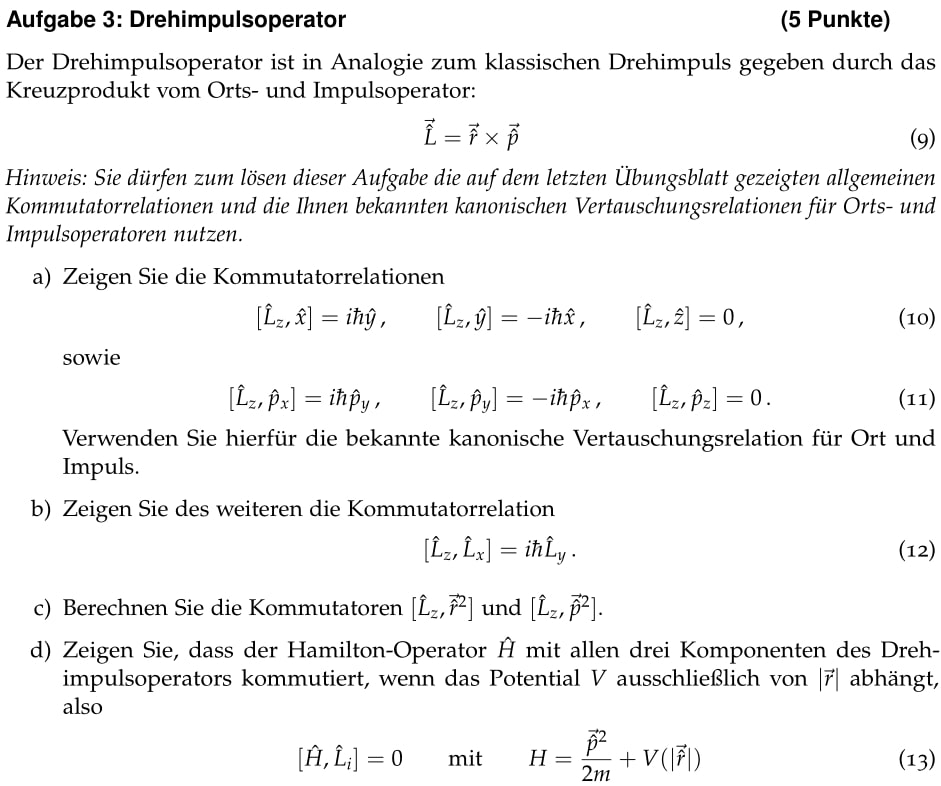
\includegraphics[width=\textwidth]{images/Aufgabe3.jpg}
        \label{fig:3}
    \end{figure}

    \subsection{a)}

    \subsection{b)}

    \subsection{c)}

    \subsection{d)}





\end{document}